\begin{figure}
	\centering
	\begin{minipage}{.4\textwidth}
		\centering
		
		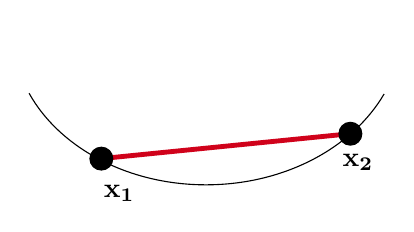
\begin{tikzpicture}[x=0.75pt,y=0.75pt,yscale=-1,xscale=1]
			\draw  [draw opacity=0, line width=1.0pt] (696.23,142.36) .. controls (681.43,167.71) and (649.5,185.54) .. (612.24,186.11) .. controls (573.51,186.7) and (539.97,168.5) .. (525.19,141.99) -- (611.08,111.08) -- cycle ; \draw   (696.23,142.36) .. controls (681.43,167.71) and (649.5,185.54) .. (612.24,186.11) .. controls (573.51,186.7) and (539.97,168.5) .. (525.19,141.99) ;
			\draw [color={rgb, 255:red, 208; green, 2; blue, 27 }  ,draw opacity=1, line width=1.75pt]   (680,161.5) -- (560,173.5) ;
			
			\draw [color={rgb, 255:red, 208; green, 2; blue, 27 }  ,draw opacity=1 ]   (680,161.5) -- (560,173.5) ;
			%Shape: Circle [id:dp3160827101885906] 
			\draw  [fill={rgb, 255:red, 0; green, 0; blue, 0 }  ,fill opacity=1 ] (554.5,173.5) .. controls (554.5,170.46) and (556.96,168) .. (560,168) .. controls (563.04,168) and (565.5,170.46) .. (565.5,173.5) .. controls (565.5,176.54) and (563.04,179) .. (560,179) .. controls (556.96,179) and (554.5,176.54) .. (554.5,173.5) -- cycle ;
			%Shape: Circle [id:dp16415395117171228] 
			\draw  [fill={rgb, 255:red, 0; green, 0; blue, 0 }  ,fill opacity=1 ] (674.5,161.5) .. controls (674.5,158.46) and (676.96,156) .. (680,156) .. controls (683.04,156) and (685.5,158.46) .. (685.5,161.5) .. controls (685.5,164.54) and (683.04,167) .. (680,167) .. controls (676.96,167) and (674.5,164.54) .. (674.5,161.5) -- cycle ;
			
			\draw (560,185) node [anchor=north west][inner sep=0.75pt]   [align=left] {$\mathbf{x_1}$};
			\draw (675,170) node [anchor=north west][inner sep=0.75pt]   [align=left] {$\mathbf{x_2}$};
		\end{tikzpicture}
		\captionof{figure}{Convex function}
	\end{minipage}%
	\begin{minipage}{.7\textwidth}
		\centering
		
		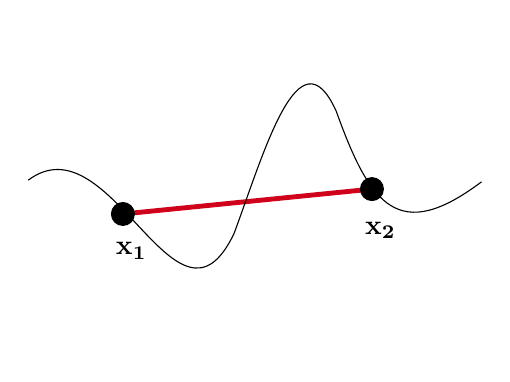
\begin{tikzpicture}[x=0.75pt,y=0.75pt,yscale=-1,xscale=1]
			%uncomment if require: \path (0,300); %set diagram left start at 0, and has height of 300
			
			%Straight Lines [id:da6875192047258083] 
			\draw [color={rgb, 255:red, 208; green, 2; blue, 27 }  ,draw opacity=1, line width=1.75pt]   (564.6,165.5) -- (444.6,177.5) ;
			%Shape: Circle [id:dp14324656781298462] 
			\draw  [fill={rgb, 255:red, 0; green, 0; blue, 0 }  ,fill opacity=1 ] (439.1,177.5) .. controls (439.1,174.46) and (441.56,172) .. (444.6,172) .. controls (447.64,172) and (450.1,174.46) .. (450.1,177.5) .. controls (450.1,180.54) and (447.64,183) .. (444.6,183) .. controls (441.56,183) and (439.1,180.54) .. (439.1,177.5) -- cycle ;
			%Shape: Circle [id:dp2582069443071713] 
			\draw  [fill={rgb, 255:red, 0; green, 0; blue, 0 }  ,fill opacity=1 ] (559.1,165.5) .. controls (559.1,162.46) and (561.56,160) .. (564.6,160) .. controls (567.64,160) and (570.1,162.46) .. (570.1,165.5) .. controls (570.1,168.54) and (567.64,171) .. (564.6,171) .. controls (561.56,171) and (559.1,168.54) .. (559.1,165.5) -- cycle ;
			%Curve Lines [id:da47039197462224447] 
			\draw    (498.2,186.8) .. controls (512.6,148) and (529.4,88) .. (547.4,128) ;
			%Curve Lines [id:da13389450894014865] 
			\draw    (399,161.2) .. controls (439,131.2) and (470.6,244.8) .. (498.2,186.8) ;
			%Curve Lines [id:da2313253314744761] 
			\draw    (547.4,128) .. controls (563.8,173.6) and (577.4,192) .. (617.4,162) ;
			
			\draw (440,190) node [anchor=north west][inner sep=0.75pt]   [align=left] {$\mathbf{x_1}$};
			\draw (560,180) node [anchor=north west][inner sep=0.75pt]   [align=left] {$\mathbf{x_2}$};
		\end{tikzpicture}
		\captionof{figure}{Non-convex function}
	\end{minipage}
\end{figure}